%%%%%%%%%%%%%%%%%%%%%%% file template.tex %%%%%%%%%%%%%%%%%%%%%%%%%
%
% This is a template file for Web of Conferences Journal
%
% Copy it to a new file with a new name and use it as the basis
% for your article
%
%%%%%%%%%%%%%%%%%%%%%%%%%% EDP Science %%%%%%%%%%%%%%%%%%%%%%%%%%%%
%
%%%\documentclass[option]{webofc}
%%% "twocolumn" for typesetting an article in two columns format (default one column)
%
\documentclass{webofc}
\usepackage[varg]{txfonts}   % Web of Conferences font

\begin{document}

\title{Track Reconstruction in the BM@N Experiment}

\author{
	\firstname{Pavel} \lastname{Batyuk}\inst{1} \and
	\firstname{Dmitriy} \lastname{Baranov}\inst{1} \and
	\firstname{Konstantin} \lastname{Gertsenberger}\inst{1} \and
	\firstname{Sergei} \lastname{Merts}\inst{1}\fnsep\thanks{\email{merts@jinr.ru}}
}

\institute{Joint Institute for Nuclear Research, Joliot-Curie, 6, 141980 Dubna, Moscow region, Russian Federation}

\abstract{The BM@N experiment (Dubna, JINR) within the NICA complex is a working experiment and it covers a wide fixed target program to be investigated.
  This work is mainly concentrated on software support of the experiment and presents a status of development and testing algorithms to be used for
  reconstruction of heavy-ion collisions. Algorithms of reconstruction are described in the work and tested with Monte Carlo input demonstrating a reasonable level of quality assurance (QA).
  First results on particle identification (PID) being a good probe to estimate quality of reconstruction are also mentioned in the work.
}

\maketitle
\section{Introduction}
\label{intro}
BM@N (Baryonic matter at Nuclotron)~\cite{bmn} is considered as a first step towards realization of physics program at the NICA complex~\cite{nica}.
It covers a fixed target program available at Nuclotron with extracted beams of different species up to gold.
The experiment had a set of technical runs mainly aimed to test sub-detector systems.
The last one took place on spring 2018 with argon and krypton beams available in a range of kinetic energies of 2.3 - 3.2 AGeV.

\begin{figure}[h]
	\centering
	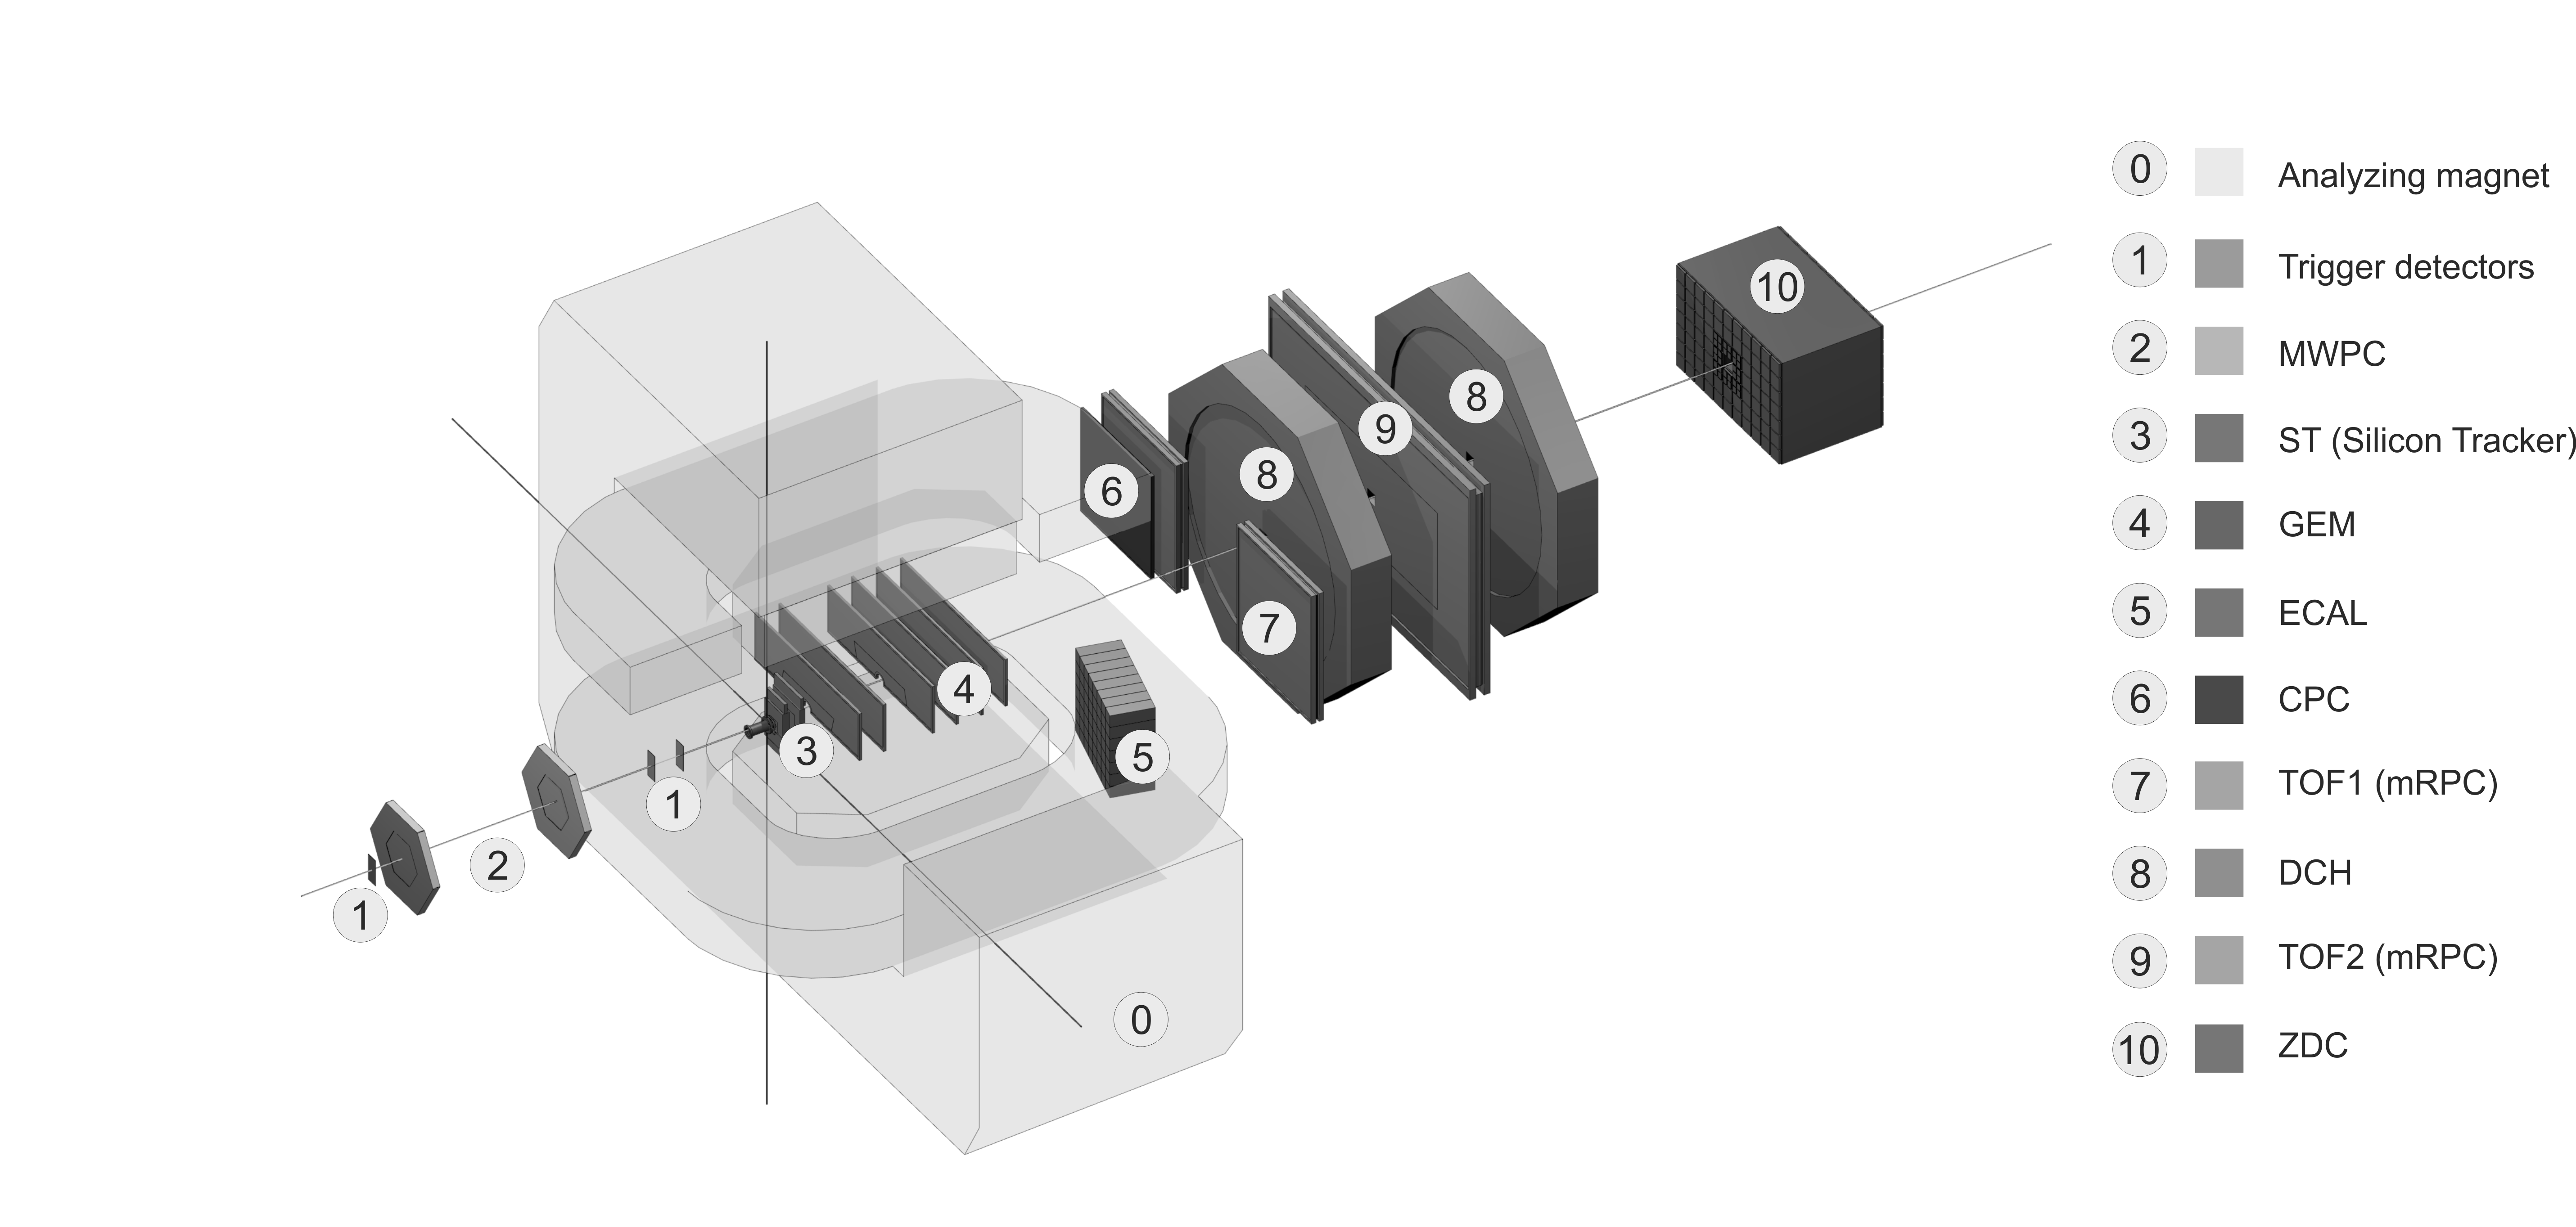
\includegraphics[width=7cm,clip]{BMN_setup_RunSpring2018_front_labels}
	\caption{BM@N experimental setup for technical run on spring 2018.}
	\label{fig-1}
\end{figure}
Reconstruction of trajectories of charged particles is considered as one of the most important and time consuming tasks in event reconstruction procedure.
An algorithm to be used when doing the procedure should be quite flexible and fast. Moreover, taking into account a different set of detectors used in all experimental
runs already performed and a fact that the last run comprised two modifications of the experimental setup, e.g., BM@N, and, in particular, Short Range Correlation Program (SRC)
at BM@N, a candidate for the algorithm should fulfil a set of requirements. The following list of options to be selected automatically within the algorithm does look obligatory: 
\begin{itemize}
	\item A modification of the experimental setup to be used, BM@N or SRC.
	\item A list of detectors to be included into the reconstruction procedure.
	\item An input data type, e.g., Monte Carlo or experimental. 
	\item Presence or absence of appropriate magnetic field, target etc.
\end{itemize}
Another important thing is related to a simple scalability of the algorithm. Indeed, a possibility to extend the algorithm for future modifications of experimental setup
with its minimal modification, in particular, in sense of the mentioned options, is considered as benefit. When searching for a candidate for the algorithm,
a huge work had been done and, finally, an algorithm based on cellular automaton~\cite{CA} was chosen. Once chosen and being tested, it was incorporated into
the BmnRoot software~\cite{soft, fairroot} to be used for its main purpose.

\section{Description of the algorithm}
\label{sec-1}
Cell is considered as a base element of the algorithm. It defined as a line segment connecting two hits pertaining to different planes of inner tracker
consisting of GEM and silicon trackers (see fig.~\ref{fig-1}). To get a more detailed description of the algorithm one is referred to~\cite{baldin}, but, nevertheless, its essence is
given here.
The algorithm consists of the following steps:
\begin{enumerate}
	\item {\bf Creation of cells.}
	  At this stage all possible connections between neighbouring detector planes are created. A restriction on maximal value of slope in ZX and ZY planes is used when creating cells. 
	\item {\bf Calculation of cell states.}
          The stage is done iteratively. At first step all cells have a state equal to unity.
          When iterating, if two cells have a common hit and similar slopes in ZX and ZY planes, then current state of right cell is increased by unity.
          Doing iterations over all elements (planes) of the inner tracker, one obtains final states for all cells.
	\item {\bf Creation of candidates to be considered as future tracks.}
	  The found cells are unified with their left neighbours if the state difference is equal to unity. As a result, an array of candidates to be considered as tracks consisting of a few cells,
	  is created. If having less than four hits, a considering candidate is rejected. The ``survived'' candidates fitted with circle are passed through procedures aimed to estimate
          vector of state and covariance matrix.
	\item {\bf Smooth of parameters of candidates.}
	  The Kalman filter is applied to the candidates aimed to improve their parameters found at the previous step.
	\item {\bf Sort of candidates.}
	  The found candidates are sorted over number of hits and using $\chi^{2}$-criterion to reject inappropriate candidates still kept at the previous steps.
	\item {\bf Selection of tracks.}
	  If two candidates sorted at the previous step have a shared hit, a candidate with a less value of $\chi^{2}$ and larger number of hits is chosen.
          The chosen candidate is considered as a track to be written to output array of found tracks.     
\end{enumerate}

\section{Testing of the algorithm}
\label{sec-2}

The developed algorithm is applicable to reconstruction of curved tracks in magnetic field as well as straight ones when there is no magnetic field.
A set of quality assurance tests performed with the Monte Carlo input containing minimal bias interactions of argon beam with kinetic energy of order of 3.2~AGeV with lead target showed
reasonable values of tracking efficiency of order of 80\% for a wide momentum range and momentum resolution (see fig.~\ref{QA}).
\begin{figure}[h]
  \centering
  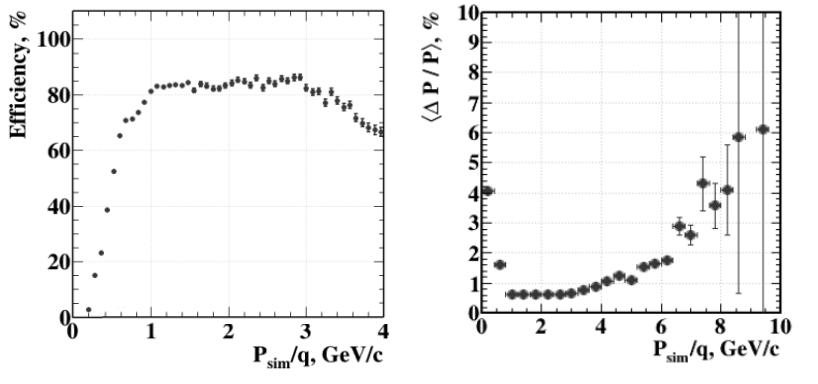
\includegraphics[width=7cm,clip]{eff_momRes_ArPb}
  \caption{Left panel: tracking efficiency as a function of momentum. Right panel: momentum resolution as a function of momentum.}
  \label{QA}
\end{figure}

A visible decrease of efficiency observed in the momentum region over 3 GeV/c could be explained by a bigger number of fragments to be if comparing with lower values of momentum. 
The fragments cross the detector just in a narrow spatial cone, thus it does not help one to understand why maximal efficiency is not higher than 80\%.
Probably, it could be explained by existing readout structure of the GEM detectors.

\section{Fake hits}
\label{sec-3}
Existing readout structure of the inner tracker leads to a big number of false strip intersections (called further ``fake hits'') due to charged particles passing through the detector
very close to each other.
For $n$ real hits and orthogonal strips the number of fake hits is calculated as $n^2 - n$. One way to decrease the number is to rotate strips of one layer at a relatively small
angle (5$^\circ$ - 15$^\circ$) with respect to another layer. This case the number of fake hits is expressed by  $(n^2 - n) \sin{\alpha}$, where $\alpha$ is an angle between strips.

Taking the Monte Carlo sample used for testing the tracking algorithm, one can estimate an average number of charged particles (having, at least, 4 hits) to be reconstructed in event (multiplicity)
equal to 50. Such ``real multiplicity'' produces a huge number of hits in the detector close to 2000. Surely, they contain an essential fraction of fake hits resulting in found track not presented
in the Monte Carlo sample. 

In fig.~\ref{fig-5} mean efficiency of track reconstruction as a function of different number of charged particles per event is shown. The framed region corresponds to ArPb-collisions.
The tracking algorithm in its current state is able to process such charged multiplicities for tracks consisting of real and, of course, fake hits, but for the well known future upgrade of the experimental
setup and use of gold ions in course of collisions planned to be studied, the algorithm requires a set of improvements. As mentioned in Section~1 and 2, the idea put in its realization allows one
to do it in existing conditions.
\begin{figure}[h]
	\centering
	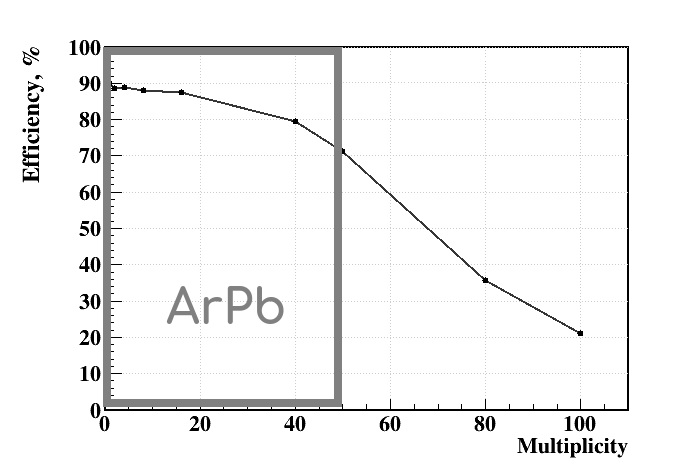
\includegraphics[width=5cm,clip]{eff_vs_mult_box_ArPb}
	\caption{Dependence of tracking efficiency on particle multiplicity in event.}
	\label{fig-5}
\end{figure}

\section{Particle identification}
\label{sec-4}
Dependence of particle velocity on particle momentum could be a good probe to get so much on quality of reconstruction due to a combined track finding efficiency and matching
of track segments from different subdetectors, e.g., the inner tracker and time-of-flight (ToF) systems. A current estimation of track parameters in the inner tracker used for matching segments with
the ToF shows a set of well distinguished lines for different types of particles (see fig.~\ref{fig-6}).
\begin{figure}[h]
	\centering
	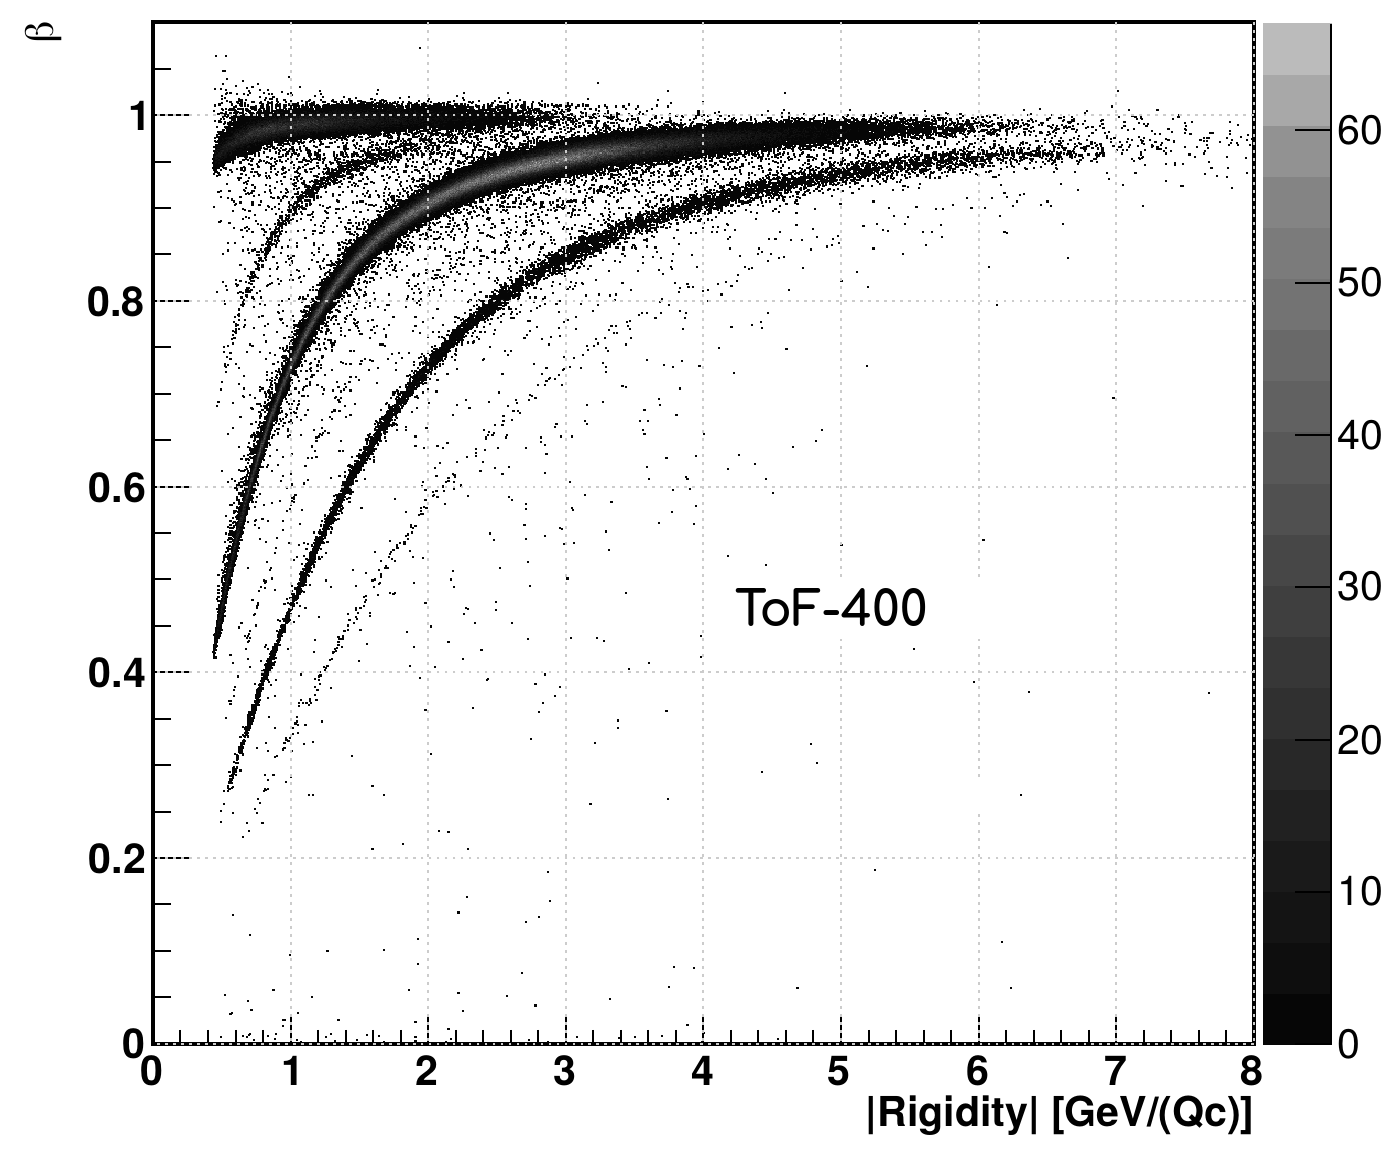
\includegraphics[width=3.5cm,clip]{pid_tof400_sim}
	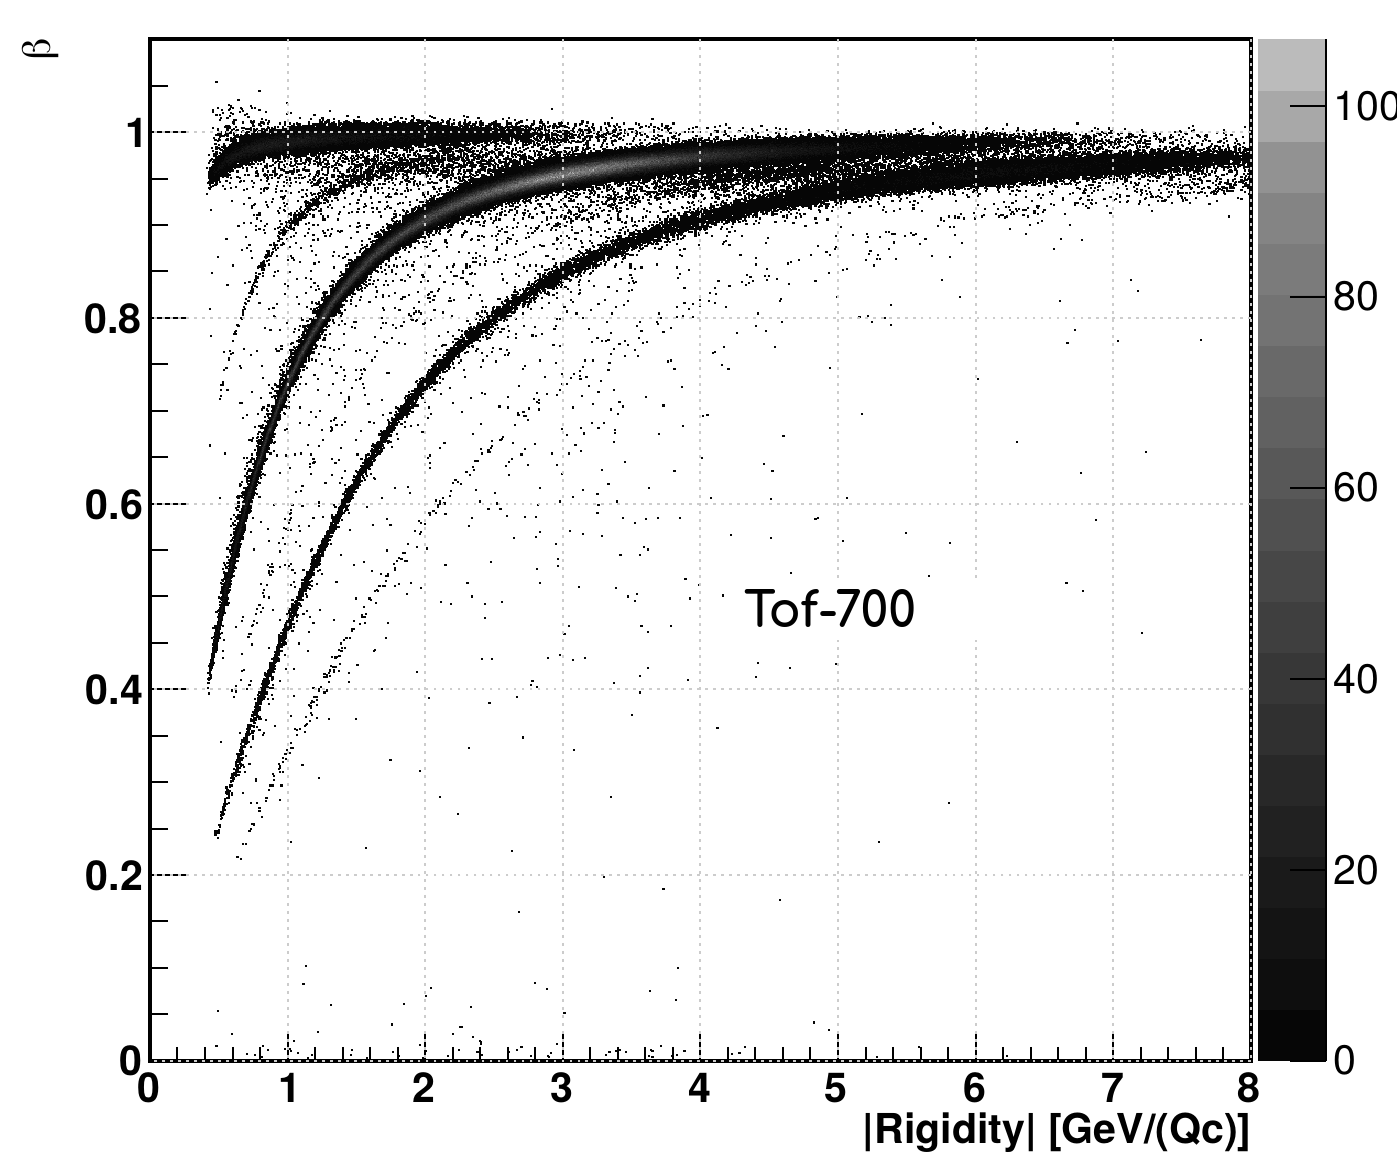
\includegraphics[width=3.5cm,clip]{pid_tof700_sim}
	\caption{Dependency of particle velocity on particle momentum.}
	\label{fig-6}
\end{figure}

\section{Acknowledgement}
This work including also a part dedicated to the development of the information systems was supported by grants of
Russian Foundation for Basic Research (18-02-40102 and 18-02-40125). We thank N. Kutovskiy and his team~\cite{jinrCloud} for possibilities to use the well equipped JINR cloud infrastructure
to perform the calculations, which were done when processing the experimental data.

\begin{thebibliography}{}
		
	\bibitem{bmn} D.~Baranov et al., KnE Energ. Phys., \textbf{3}, 291-296 (2018)
	\bibitem{nica} V.~Kekelidze, JINST, \textbf{12}, 06012 (2017)
	\bibitem{CA} R.~Glattauer et al., arXiv:1202.2761
	\bibitem{baldin} P.~Batyuk et al., EPJ~Web~of~Conferences \textbf{204}, 7012 (2019)
	\bibitem{fairroot} M.~Al-Turany et al., J.~Phys.: Conf.~Ser., \textbf{396}, 022001 (2012)
	\bibitem{soft} K.~Gertsenberger et al., Eur.~Phys.~J.~A., \textbf{52}, 16214 (2016)
        \bibitem{jinrCloud} A.~V.~Baranov, N~A.~Balashov, N.~A.~Kutovskiy, R~N.~Semenov, Physics of Particles and Nuclei Letters 13(5), 672 (2016)
	
\end{thebibliography}

\end{document}

% end of file template.tex


